\documentclass[8pt]{article}

\usepackage[T1]{fontenc}
\usepackage[utf8]{inputenc}
\usepackage{graphicx}
\usepackage{lmodern}
\usepackage{amsmath}
\usepackage{xfrac}
\usepackage{amsthm}
\usepackage{listings}
\usepackage{enumerate}
\usepackage{amssymb}
\usepackage{cancel}
\usepackage{amsfonts}
\usepackage{float}
\usepackage{fullpage}
\usepackage{pdfpages}
\usepackage{tcolorbox}

\DeclareUnicodeCharacter{200A}{ } 
\renewcommand*\contentsname{Table des matières}

\PassOptionsToPackage{hyphens}{url}\usepackage{hyperref}

\usepackage{listings}
\author{ControverSciences\textit{ et al} }
\title{Projet AREN - Corpus de ressources. \\ Essence \& Diesel.}
\date{7 Février 2020}

\begin{document}
\maketitle

Les sujet de la pollution à l'essence et au diesel est abordé par les définitions des moteurs à essence \& diesel ainsi que des données sur leurs performances (\ref{sec:essencediesel}). Ensuite les rumeurs, et les vrai-faux concernant leurs pollutions respectives sont analysées dans 2 articles du journal \textit{Le Monde}, en 2018 (\ref{sec:lemonde_vraifaux}) et 2019 (\ref{sec:lemonde_moinspolluant}). Enfin deux articles de synthèses viennent replacer les pollutions des moteurs dans un contexte plus générale de pollution des voitures (\ref{sec:conversation_voitures}) et de la pollution de l'air en générale (\ref{sec:converstion_air}).\\

Ce corpus de préparation permet d'aborder les différentes facettes du sujet de la pollution à l'essence et au diesel, afin de débattre sur le scandale du DieselGate (\ref{debat:dieselgate}), ou bien sur la nocivité de l'essence (\ref{debat:essencepire}).

\tableofcontents

\newpage
\section{Textes à débattre}

\subsection{Le dieselgate, un scandale industriel bien encombrant}
\label{debat:dieselgate}

\begin{itemize}
	\item \textbf{Lien~: } \url{https://www.lepoint.fr/automobile/securite/le-dieselgate-un-scandale-industriel-bien-encombrant-18-06-2018-2228231_657.php} 
	\item \textbf{Date~: } 18 juin 2018
	\item \textbf{Source~: } Le Point est un magazine français d'actualité hebdomadaire de dimension nationale. Depuis 1997, il appartient à la famille Pinault, qui détient à 100\% le groupe via une holding. 
\end{itemize}

Après avoir éclaté aux États-Unis, l'affaire des moteurs truqués revient en force en Allemagne avec des dégâts collatéraux dont on peine à mesurer l'ampleur. Le scandale des moteurs diesel truqués, pour lequel le patron d'Audi, filiale de Volkswagen, a été incarcéré lundi en Allemagne, éclabousse depuis trois ans l'ensemble de l'industrie automobile mondiale.\\

Le 18 septembre 2015, l'agence environnementale américaine (EPA) accuse Volkswagen (VW) d'avoir installé un «~logiciel truqueur~» sur des centaines de milliers de véhicules diesel fabriqués à partir de 2009 pour les faire paraître moins polluants qu'ils ne le sont réellement.
Le logiciel enclenche un mécanisme interne de limitation des gaz polluants pendant les contrôles. Les enquêteurs découvrent que les émissions réelles d'oxyde d'azote – un gaz à l'origine de maladies respiratoires et cardiovasculaires – sont jusqu'à quarante fois supérieures à la limite légale.
VW reconnaît avoir truqué 11 millions de véhicules diesel, dont 8,5 millions en Europe et 600 000 aux États-Unis. Ces véhicules portent pour la plupart la marque Volkswagen, mais la tricherie concerne également d'autres marques du groupe comme Audi, Porsche, Seat et Skoda.\\

Les conséquences pécuniaires pour les propriétaires de voitures incriminées sont très différentes des deux côtés de l'Atlantique. Aux États-Unis, où les normes antipollution sont plus strictes, le groupe a accepté de réparer ou racheter près de 600 000 voitures et d'indemniser leurs propriétaires.
Mais en Europe, où a été vendue la grande majorité des voitures truquées, VW n'a pas dédommagé ses clients, car la situation et la législation y sont, selon lui, différentes de celles rencontrées aux États-Unis. S'il y a, en effet, une approche différente des mesures de pollution, cela n'entame en rien la présomption de fraude d'un logiciel modifiant les mesures. En d'autres termes, le coup de tampon de l'homologation est bien là, mais la morale, elle, n'est pas respectée.\\

En Allemagne, plusieurs enquêtes ont été ouvertes pour fraude, manipulation de cours ou publicité mensongère. Deux hauts responsables du groupe Volkswagen ont été incarcérés~: le patron d'Audi, en juin, et un haut responsable de Porsche, en avril. Le chef du développement des moteurs chez Audi de 2001 à 2007, est également en détention. Aux États-Unis, Volkswagen a accepté de payer plus de 22 milliards de dollars pour contenter autorités, clients et concessionnaires. Le groupe a également accepté une amende d'un milliard d'euros en Allemagne.
VW n'encourt plus de poursuites judiciaires de la part des autorités américaines, mais les employés du groupe à titre individuel restent menacés. Huit anciens et actuels dirigeants de Volkswagen et un cadre d'Audi ont été inculpés. Parmi eux, deux ont déjà été condamnées à des peines de prison.\\

Des tests menés après la découverte du dieselgate ont permis d'établir que les moteurs diesel d'autres constructeurs s'avéraient également plus polluants dans la réalité que lors des contrôles. Ce qui est parfaitement normal tant il y a un gouffre entre la méthode de mesure en usage avant et celle mise en œuvre maintenant et reflétant de plus près la réalité.
Ainsi, sur ces différents cas et dans l'attente d'autres investigations, il n'existe à ce stade aucun élément permettant de conclure formellement à des fraudes. Tout juste peut-il s'agir d'optimisation des moteurs, la flexibilité de l'électronique faisant varier de nombreux paramètres en fonction des critères de roulage du moment. Les constructeurs ont même argué que les réglementations les autorisaient, dans certaines circonstances, à désactiver les systèmes de contrôle des émissions polluantes pour protéger le moteur. 

\newpage
\subsection{L’essence est le pire carburant pour votre santé}
\label{debat:essencepire}

\begin{itemize}
	\item \textbf{Lien~: } \url{https://www.anthropocenemagazine.org/2017/07/lessence-est-le-pire-carburant-pour-votre-sante/?lang=fr} 
	\item \textbf{Auteur~: } Prachi Patel, journaliste scientifique.
	\item \textbf{Date~: } 20 juillet 2017
	\item \textbf{Source~: } \textit{Anthropocene} est un magazine (numérique \& imprimé) à l'initiative de Future Earth, un consortium scientifique, dont la mission est d'organiser une conversation mondiale sur les données, la technologie et l'innovation qui mènent à des solutions aux défis environnementaux persistants de notre époque.
\end{itemize}

Deux études récentes exposent le désavantage des voitures fonctionnant à l’essence par rapport à d’autres combustibles liquides. Elles démontrent que les voitures à essence sont plus problématiques en ce qui concerne la pollution par les particules de carbone. Les résultats indiquent que renoncer à l’essence sera bon pour l’environnement et la santé humaine.\\

L’une des études a analysé des données sur la taille des particules polluantes, des données météorologiques, le trafic automobile et le comportement des consommateurs. Ils ont constaté que le choix de carburant n’a pas affecté la concentration de plus grosses particules, entre 100 nanomètres et 2,5 micromètres de diamètre, qui sont réglementées aux États-Unis et dans d’autres pays.
Cependant, les particules ultrafines (de 7 à 100 nanomètres de diamètre), qui ont fluctué avec le choix du carburant, passent sous le radar. «~La tendance observée dans les grandes villes à délaisser l’essence en faveur de véhicules alimentés par l’éthanol, l’électricité, ou un mélange des deux, entraînera une réduction de ces particules ultrafines~», a déclaré Franz Geiger, professeur de chimie à la Northwestern dans un communiqué de presse. «~Cela s’accompagne probablement d’un avantage pour la santé — ces particules, inférieures à un micron, ont le potentiel de s’introduire profondément dans vos poumons~».\\

La seconde étude, quant à elle démontre que les voitures diesel modernes émettent généralement moins de particules de carbone que les voitures à essence.
Les vieux moteurs diesel sont reconnus pour exhaler des gaz toxiques contenant des polluants tels que le dioxyde de soufre, des oxydes d’azote et des particules de carbone. Les voitures diesel ont également été critiquées avec le récent scandale de la tromperie sur les émissions de Volkswagen.
Mais la nouvelle étude démontre que les voitures diesel ne sont pas les vilains coupables que nous en avons faits. Les plus récents moteurs diesel en Europe et en Amérique du Nord sont plus propres parce qu’ils doivent être équipés de filtres à particules. Lesquelles des voitures à essence ou au diesel sont plus polluantes dépend du polluant en question.
L'étude a constaté que les voitures à essence ont émis en moyenne dix fois plus de particules de carbone, et 62 fois plus à -7 °C, par rapport aux voitures diesel. Cependant, les voitures diesel ont émis dix fois plus d’oxydes d’azote aux deux températures.\\

Cela signifie que les passagers ont le choix entre des voitures qui émettent généralement moins de particules (diesel), ou des voitures qui émettent moins d’oxydes d’azote (essence). «~Les voitures diesel ne sont pas forcément plus polluantes que les voitures à essence~», écrivent les chercheurs.
La meilleure option est peut-être de tout simplement abandonner les voitures, soutient un éditorial paru dans Nature.

\newpage
\section{Corpus de ressources}

\subsection{Les véhicules essence et Diesel}
\label{sec:essencediesel}

\begin{itemize}
	\item \textbf{Lien~: } \url{https://www.ifpenergiesnouvelles.fr/enjeux-et-prospective/decryptages/transports/les-vehicules-essence-et-diesel} 
	\item \textbf{Auteur~: } Institut Français du Pétrole Énergies nouvelles (IFPEN)
	\item \textbf{Date~: } 26 octobre 2018
	\item \textbf{Date~: } L'IFPEN un établissement public national à caractère industriel et commercial avec des missions de recherche et de formation. Il a pour objectif d'assurer, dans les domaines de l’énergie, du transport et de l’environnement, le développement des technologies et matériaux du futur
\end{itemize}

Depuis son invention, l’automobile fonctionne majoritairement à l’aide d’un moteur thermique à combustion interne, à 4 temps. En Europe, il est surtout alimenté à l’essence (moteur à allumage commandé) ou au gazole (moteur Diesel).
Des progrès technologiques importants ont permis d’augmenter le rendement des moteurs thermiques en vue de réaliser des économies d’énergie et de diminuer très fortement les émissions de polluants. La préoccupation écologique est au cœur de la recherche sur le développement des moteurs.Les performances d'un moteur dépendent, en premier lieu, de la quantité d'énergie dégagée par la combustion, donc de la quantité de mélange carburé présente dans la chambre de combustion. Celles-ci sont ainsi directement liées au volume de la chambre (cylindrée unitaire), au nombre de chambres ou cylindres du moteur (cylindrée totale) et à la quantité de carburant injecté.\\

\textbf{Pourquoi l’appellation "moteur à 4 temps"~?}\\

Ce sont les 4 temps nécessaires au cycle de transformation de l'énergie chimique contenue dans le carburant en énergie mécanique. Chaque temps correspond à un demi-tour de rotation du vilebrequin (une montée ou une descente du piston). Les temps 1 et 4 sont consacrés aux transferts des gaz (admission des gaz frais et échappement des gaz brûlés), les temps 2 et 3 sont les temps nécessaires à la préparation et à la réalisation de la combustion et à sa transformation en énergie mécanique. Pour un moteur à allumage commandé et à injection indirecte, les 4 temps sont~:
\begin{enumerate}
	\setlength\itemsep{-0.1em}
	\item Admission (remplissage du cylindre). Le piston descend et aspire le mélange air-carburant. 
	\item Compression. Le piston remonte comprimant le mélange air-carburant, une étincelle est générée pour enflammer le mélange.
	\item Combustion-Détente. Ce temps correspond au développement de la combustion et à l'expansion des gaz brûlés~: le piston est repoussé vers le bas, l’énergie chimique est transformée en énergie mécanique.
	\item Échappement (vidange des gaz brûlés du cylindre). Le piston remonte et évacue les gaz brûlés.
\end{enumerate}
\begin{center}
	\makebox[\textwidth]{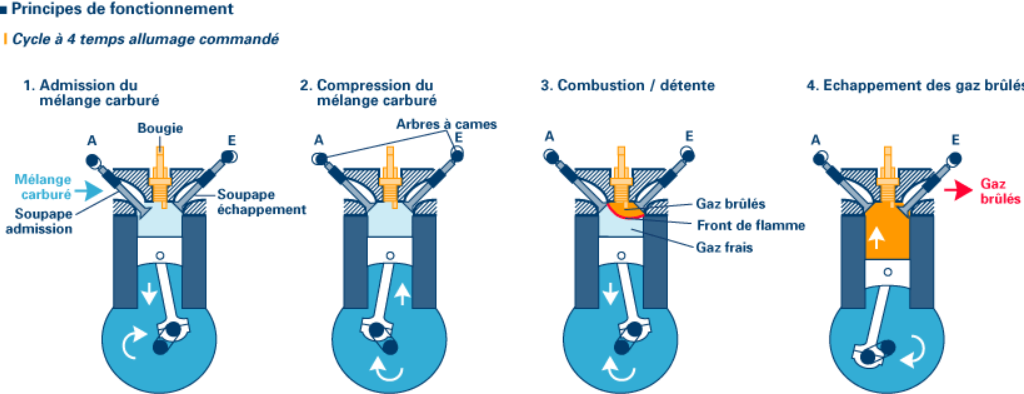
\includegraphics[width=\textwidth]{essence-diesel-fig-1}}
\end{center}

Pour un moteur Diesel à allumage par compression et injection directe, les 4 temps se déroulent de la même façon à deux différences près~:
\begin{itemize}
	\setlength\itemsep{-0.1em}
	\item c'est de l'air pur qui est admis et comprimé lors des temps 1 et 2, puis le carburant est introduit directement dans le cylindre (par injection) en fin de compression,
	\item le mélange s’enflamme spontanément, sans étincelle, du fait de l'élévation de la température de l'air liée à sa compression.
\end{itemize}

\textbf{Qu'est-ce que la combustion~?}\\

Pour réaliser une combustion complète d'1 g de carburant conventionnel (essence ou gazole), il faut, en théorie, environ 14,6 g d'air. Ce mélange idéal est appelé mélange stœchiométrique.
Les moteurs à essence à injection indirecte fonctionnent en grande majorité à la stœchiométrie. Après introduction d'un mélange homogène d'air et d'essence dans le moteur, la combustion (inflammation du mélange) est initiée par une étincelle (allumage commandé). La combustion se traduit par la propagation d'un front de flamme qui balaye toute la chambre.
Les moteurs à essence actuels à injection directe~: l’air arrive par l’admission et le carburant, comme dans un moteur Diesel, arrive directement dans la chambre de combustion, ce qui permet un pilotage plus précis des injections. Il n’y a plus de prémélange air-carburant, il s’agit alors d’un mélange dit stratifié. La combustion est toujours initiée par une étincelle (allumage commandé).
Les moteurs Diesel fonctionnent avec un excès d'air. Le gazole est injecté sous pression dans une masse d'air préalablement comprimée. La combustion s'initie par auto-inflammation (allumage par compression). La combustion est dite stratifiée ou hétérogène car elle a lieu dans un milieu constitué à la fois de zones très riches en carburant (situées notamment près du nez d'injecteur) et de zones très pauvres (près de la paroi du cylindre).\\

\textbf{Les carburants} \\

En Europe, l’essence alimente les moteurs à allumage commandé et le gazole les moteurs Diesel. Ce sont les deux principaux produits finis issus du raffinage du pétrole brut et leur formulation évolue avec les exigences des moteurs et surtout avec les réglementations environnementales liées à la qualité de l’air et à la réduction des rejets de gaz à effet de serre.\\

\newpage
\textbf{Qu’est-ce que le rendement d’un moteur~?}\\

Le moteur est un transformateur d'énergie chimique en énergie mécanique. Le rendement d’un moteur est le rapport entre l’énergie fournie au moteur (énergie chimique contenue dans le carburant) et l’énergie mécanique restituée. Il est important d’optimiser ce rendement pour éviter la déperdition d’énergie, particulièrement dans un contexte de développement durable. Dans des conditions optimales de fonctionnement, un moteur automobile offre aujourd'hui un rendement maximal~:
\begin{itemize}
	\setlength\itemsep{-0.1em}
	\item de l'ordre de 36\% pour un moteur à essence,
	\item et de 42\% pour un moteur Diesel.
\end{itemize}

C’est-à-dire que dans les points de fonctionnement les plus favorables, un peu plus d'un tiers de l'énergie fournie par le carburant est transformée en énergie utile pour faire avancer le véhicule, le reste étant principalement dissipé en chaleur dans l'atmosphère. Ces conditions optimales correspondent cependant à une utilisation du moteur à charge élevée.
La puissance maximale que doit fournir le moteur est déterminée par~:
\begin{itemize}
	\setlength\itemsep{-0.1em}
	\item la masse du véhicule,
	\item sa vitesse maximale,
	\item et son agrément d'utilisation (lutte contre l’inertie liée au poids, résistance à l'avancement dans l'air, potentiel d'accélération).
\end{itemize}

Or, en règle générale, les véhicules automobiles sont utilisés sur de petits parcours en agglomération, ce qui se traduit finalement par une sollicitation des moteurs à faibles charges. Dans ces conditions, le rendement se trouve dégradé avec des valeurs n'atteignant que 15\%.
De gros efforts de recherche et développement sont engagés dans ce domaine afin d'améliorer les rendements des moteurs dans toutes les conditions d'utilisation des véhicules.\\

\textbf{Le post-traitement des émissions polluantes}\\

C’est l’étape qui consiste à transformer les gaz d'échappement, entre le moteur et le pot d’échappement, pour obtenir des émissions de gaz moins polluants.
Actuellement, il existe deux principaux moyens pour réaliser le post-traitement des émissions~:
\begin{itemize}
	\setlength\itemsep{-0.1em}
	\item le pot catalytique qui convertit principalement le CO, les HC et les NOx, et qui permet de réduire également les particules de suie (fraction organique soluble présente sur les particules),
	\item le filtre à particules qui stocke les particules, puis les brûle périodiquement (tous les 500 km environ) dans des conditions parfaitement maîtrisées.
\end{itemize}

D’autres technologies sont mises en œuvre pour améliorer encore le traitement des émissions, parmi lesquelles on peut citer, les pièges à oxyde d'azote et la catalyse "SCR" (avec injection d'un agent réducteur spécifique, l'urée).


\newpage
\subsection{Le vrai du faux sur la pollution des voitures au diesel}
\label{sec:lemonde_vraifaux}

\begin{itemize}
	\item \textbf{Lien~: } \url{https://www.lemonde.fr/les-decodeurs/article/2018/10/26/le-vrai-du-faux-sur-la-pollution-des-voitures-au-diesel_5374931_4355770.html} 
	\item \textbf{Auteur~: } Adrien Sénécat
	\item \textbf{Date~: } 26 octobre 2018.
	\item \textbf{Source~: } Le Monde est un journal français à la ligne éditoriale parfois présentée comme étant de centre gauche, bien que cette affirmation soit récusée par le journal lui-même, qui revendique un traitement non partisan. Le journal est édité par le groupe Le Monde, détenu à 72,5\% par la société Le Monde libre, elle-même contrôlée à parité par les hommes d'affaires Xavier Niel et Matthieu Pigasse.
\end{itemize}

«~Matraquage fiscal~», «~hold-up~», «~scandale~»…, des dizaines de pétitions, vidéos ou messages largement partagés sur les réseaux sociaux s’insurgent depuis plusieurs semaines contre la hausse des prix à la pompe, en particulier du diesel depuis que le coût de celui-ci a rejoint celui de l’essence.
Face aux critiques, le gouvernement justifie son choix d’augmenter sensiblement les taxes sur les carburants, en particulier sur le diesel, par des considérations environnementales. Pourtant, une bonne partie des sceptiques remettent en cause cet argument, arguant notamment du fait que les dangers du diesel seraient «~exagérés~». A tort ou à raison~? Nous avons passé en revue quatre arguments récurrents de ce débat pour tenter d’y voir plus clair.\\

\textbf{1. «~Les voitures qui roulent au diesel émettent moins de CO$_2$ que celles qui roulent à l’essence~».} C’EST PLUS COMPLIQUÉ\\

A première vue, les faits peuvent sembler clairs~: la consommation moyenne de carburant d’un véhicule diesel (6,07 litres pour 100 km parcourus) est sensiblement moindre que celle d’une voiture à essence (7,31), selon les chiffres du ministère de l’environnement pour l’année 2017. On peut donc s’attendre à un plus faible rejet de CO$_2$, un gaz à effet de serre.
Plusieurs facteurs compliquent néanmoins l’équation. D’abord, un litre de gazole brûlé rejette en moyenne plus de CO$_2$ qu’un litre d’essence (de l’ordre de 2,6 kilos par litre contre 2,3 environ pour l’essence). Surtout, une analyse exhaustive ne doit pas se limiter à la pollution émise lorsque la voiture est utilisée, mais à son cycle de vie complet, qui inclut également sa fabrication et sa durée de vie.\\

Une étude de l’ONG Transport \& Environment a tenté en 2017 de tenir compte de ces facteurs, aboutissant à la conclusion inverse de celle communément admise~: sur l’ensemble de sa vie, une voiture au diesel rejetterait finalement autour de 10\% de CO$_2$ de plus qu’une essence (42,65 tonnes contre 39).
Mais cette étude elle-même présente des limites. Notamment du fait que, en comparant la voiture diesel moyenne avec sa rivale essence moyenne, elle a mis en balance deux véhicules aux profils différents (en moyenne, les véhicules diesel en circulation sont plus imposants que les véhicules à essence). Elle a aussi tenu compte du fait que les moteurs au gazole font plus de kilomètres (de l’ordre de 4\%) que ceux à essence, du fait notamment que le diesel était moins cher à la pompe, ce qui n’est désormais plus le cas. Il est donc fort possible que les pratiques des conducteurs évoluent.
Malgré ces bémols, l’étude de Transport \& Environment montre tout de même que l’avantage du gazole s’agissant d’émission de CO$_2$ est finalement moins évident qu’on pourrait le croire.\\

\textbf{2. «~Le diesel pollue globalement moins que l’essence~».} C’EST FAUX\\

C’est pourtant ce que martèlent certains. Un message partagé plus de 50 000 fois sur Facebook au mois d’octobre affirme ainsi que puisqu’un véhicule diesel produit en moyenne moins de CO$_2$ à distance parcourue égale, il «~pollue moins~» que l’essence. Ce raisonnement est en réalité simpliste, non seulement parce qu’il met de côté le reste du cycle de vie des véhicules, mais surtout parce qu’il occulte le principal reproche formulé à l’encontre des voitures au diesel.\\

Ce ne sont en effet pas tant les émissions de CO$_2$ que celles de particules fines et d’oxyde d’azote (NOx) qui sont pointées du doigt dans le cas du diesel. Or, celles-ci ont des conséquences néfastes pour la santé, notamment sur les voies respiratoires, et en particulier dans les grandes agglomérations comme Paris, où une bonne partie de la population réside à proximité d’un axe routier.
Une étude publiée en 2017 dans la revue Environmental Research Letters estimait que sur 425 000 morts prématurées par an associées à la pollution de l’air dans en Europe, environ 10 000 peuvent être attribuées directement aux émissions de NOx des moteurs diesel.\\

\textbf{3. «~Les véhicules diesel récents ont réglé le problème~».} C’EST PLUS COMPLIQUÉ\\

Il s’agit là encore d’un argumentaire souvent mis en avant par les industriels et très populaire sur les réseaux sociaux. Un message partagé plus de 600 000 fois sur Facebook affirme ainsi que les voitures qui roulent aujourd’hui au diesel «~sont équipées de filtres qui piègent ces particules fines à hauteur de 99,9\%, c’est-à-dire qu’elles n’en rejettent quasiment plus du tout~».
Le constat de fond est plutôt juste~: les véhicules les plus récents polluent globalement moins que les vieilles voitures. Concernant le diesel, les normes européennes (Euro 1, puis Euro 2, et désormais Euro 6) en vigueur n’ont fait que se durcir depuis leur apparition dans les années 1990.\\

Cependant, la pratique est souvent éloignée de la théorie. D’abord dans des cas de tricherie avérée comme le «~dieselgate~» où les normes ont été bafouées. Mais aussi, plus largement, dans des cas d’optimisation où des véhicules ont pu répondre correctement aux tests d’émission alors qu’ils polluent nettement plus en conditions réelles. Même les moteurs qui répondent aux normes Euro 6 polluent ainsi bien plus qu’annoncé, selon une étude de l’Agence fédérale allemande pour l’environnement publiée en avril 2017.
Enfin, des inquiétudes subsistent. En février 2018, ce sont des particules ultrafines (d’un diamètre inférieur à 0,1 µm) qui ont été pointées du doigt dans un article de Thomas Bourdrel, un médecin radiologue de Strasbourg, dans la revue Réalités cardiologiques. Selon ce dernier, 90\% des particules émises par les moteurs diesel de dernière génération se rangent dans cette catégorie, alors qu’elles sont les plus dangereuses en raison de leur taille et de leur composition.
Tous ces éléments montrent qu’il est donc au minimum audacieux d’affirmer que le problème serait complètement «~réglé~».\\

\textbf{4. «~Le système de bonus-malus écologique favorise le diesel~».} C’EST VRAI\\

C’est notamment ce qu’a affirmé Pierre Chasseray, délégué de l’association 40 millions d’automobilistes, sur Sud Radio le 8 octobre~: «~Le système de bonus-malus est basé uniquement sur les émissions de CO$_2$, et le meilleur en termes d’émission de CO$_2$, c’est le diesel, donc forcément les véhicules qui bénéficieront de malus neutres, ce sont les petites voitures diesel urbaines.~»
Le dispositif du bonus-malus écologique est simple sur le papier. Il cumule deux mesures, présentées de la sorte sur le site du ministère de l’économie~:
\begin{itemize}
	\setlength\itemsep{-0.1em}
	\item «~Un bonus pour l’acquisition de véhicules propres, assorti d’une prime pour la destruction d’un véhicule ancien ;
	\item Un malus applicable aux voitures particulières les plus polluantes, ainsi qu’une taxe annuelle pour certains modèles~»
\end{itemize}

Or, les deux pans de la mesure sont basés sur les émissions de CO$_2$ rapportées en gramme par kilomètre. On l’a vu, les diesels sont effectivement moins polluants sur ce strict terrain (cet avantage est néanmoins contesté si l’on prend en compte l’intégralité de leur cycle de vie). A modèle égal, les véhicules diesel sont donc bien fiscalement favorisés par rapport à leur version essence, ce qui peut sembler quelque peu paradoxal.
Alors que l’actuel ministre de l’environnement, François de Rugy, proposait lui-même dans son programme pour la primaire de la gauche en 2017 de «~proscrire~» la vente de véhicules diesel dès 2025, ces derniers sont encore aujourd’hui en partie subventionnés par un dispositif qui se veut vertueux en matière d’environnement.

\newpage
\subsection{Non, le diesel n’est pas finalement «~moins polluant que l’essence~»}
\label{sec:lemonde_moinspolluant}
\begin{itemize}
	\item \textbf{Lien~: } \url{https://www.lemonde.fr/les-decodeurs/article/2019/02/15/non-le-diesel-n-est-pas-finalement-moins-polluant-que-l-essence_5424021_4355770.html} 
	\item \textbf{Auteur~: } Adrien Sénécat
	\item \textbf{Date~: } 15 février 2019
	\item \textbf{Source~: } Le Monde est un journal français à la ligne éditoriale parfois présentée comme étant de centre gauche, bien que cette affirmation soit récusée par le journal lui-même, qui revendique un traitement non partisan. Le journal est édité par le groupe Le Monde, détenu à 72,5\% par la société Le Monde libre, elle-même contrôlée à parité par les hommes d'affaires Xavier Niel et Matthieu Pigasse. Il bénéficie de subventions de la part de l'État français.
\end{itemize}

A en croire des gros titres publiés ces derniers jours, la conclusion est sans appel~: le diesel est finalement «~moins polluant que l’essence~». L’information a de quoi faire sursauter quiconque s’intéresse à l’écologie ou au débat sur les prix des carburants ces derniers mois. Pour défendre l’alignement de la fiscalité du gazole sur celle de l’essence, qui a contribué à déclencher le mouvement des «~gilets jaunes~», le gouvernement – et celui qui l’a précédé – fondait précisément sa politique sur le fait que le diesel polluerait plus.
Sauf qu’à y regarder de plus près, cette controverse est beaucoup trop complexe pour être résumée de la sorte. Alors, qui enfume qui~? Et que penser de la pollution des voitures à essence et diesel~?\\

\textbf{Ce que dit la rumeur}\\

Tout est en fait parti d’un sujet du journal de 13 heures de TF1 le 7 février. «~Peut-être l’avez-vous entendu ce matin, le ministère de l’économie ne serait pas contre un retour en grâce du diesel~», y affirme le présentateur, Jean-Pierre Pernaut. «~Les moteurs diesel modernes ne pollueraient pas tant que ça et même moins que les voitures à essence. Tiens donc, on vous disait le contraire il y a quelques mois~», ironise ensuite le journaliste.
Le reportage qui suit donne la parole à des automobilistes quelque peu déroutés, qui ne savent plus vraiment quel type de véhicule pollue, ni pourquoi. L’extrait, repris sur la page Facebook La France des actes, a été visionné plus de 160 000 fois sur le réseau social en une semaine.
Et plusieurs sites internet ont rapidement saisi la balle au bond~: «~deux mois après, Bercy explique que le diesel serait… finalement moins polluant que l’essence~!~» et «~non, ce n’est pas Le Gorafi~», s’esclaffe le site revolutionpermanente.fr dans un article partagé plus de 30 000 fois sur Facebook. L’article conclut que la «~propagande anti-diesel~» est une «~supercherie totale~».\\

POURQUOI C’EST FAUX\\

\textbf{1. Au départ, une réflexion qui divise au sein du gouvernement}\\

Le sujet du JT de 13 heures de TF1 part d’une information avérée~: le gouvernement envisage actuellement ce qu’on peut présenter comme une réhabilitation partielle du diesel, en tout cas des véhicules les plus récents. Elle consisterait en une évolution de la classification Crit’Air, du nom de ces vignettes à apposer sur le pare-brise des véhicules et qui les classent en fonction de leurs émissions de polluants atmosphériques.
Il existe cinq classes de véhicules Crit’Air. Jusqu’à présent, les véhicules qui roulent au gazole étaient bannis de la classification Crit’Air 1, la mieux disante de toutes. C’est sur cette règle que le gouvernement envisage aujourd’hui de revenir, en rendant les véhicules diesel les plus récents éligibles à Crit’Air 1.
La décision de faire évoluer ou non la classification Crit’Air pose de réels enjeux, puisque c’est sur elle que se basent certaines villes pour interdire aux véhicules les plus polluant de circuler. A Paris, par exemple, seuls les particuliers dont la voiture a une vignette Crit’Air 4 ou mieux peuvent circuler du lundi au vendredi de 8 heures à 20 heures. Et la capitale prévoit d’interdire progressivement la circulation de tous les diesels d’ici à 2024. Sauf que les diesels les plus récents pourraient passer entre les mailles du filet si le gouvernement les rendait éligibles à la vignette Crit’Air 1.
Cette piste n’est pour l’heure qu’à l’étude et «~fait l’objet de discussions serrées entre les différents ministères concernés~», révélait récemment Le Monde. Mais «~le ministère de l’écologie est contre~», a assuré la secrétaire d’Etat Emmanuelle Wargon sur RTL le 7 février.\\

\textbf{2. Que sait-on de la pollution des véhicules au diesel~?}\\

Le débat sur la pollution liée au diesel est en réalité truffé de pièges, car tout dépend de quel type de polluant on parle. Si l’on se focalise sur les gaz à effet de serre (à commencer par le CO$_2$), il est couramment admis que les véhicules diesel en rejettent un peu moins que leurs équivalent à essence, car moins consommateurs de carburant. C’est notamment pour cela que le diesel a un temps été favorisé par les pouvoirs publics.
Le problème, c’est que le diesel présente un inconvénient majeur si l’on s’intéresse cette fois aux particules fines et aux oxydes d’azote (NOx). Ces polluants ont des conséquences néfastes pour la santé, notamment pour les personnes qui résident à proximité d’un axe routier.
Ainsi, une étude publiée en 2017 dans la revue Environmental Research Letters estimait que sur 425 000 morts prématurées par an associées à la pollution de l’air en Europe, environ 10 000 peuvent être attribuées directement aux émissions de NOx des moteurs diesel. C’est sur cette base que l’on entend régulièrement que le diesel «~pollue plus~» que l’essence, même si cette formule est quelque peu hâtive.\\

\textbf{3. Les diesels récents échappent-ils à la règle~?}\\

Les normes européennes imposées aux véhicules diesel et essence se sont sensiblement renforcées au fil des ans depuis leur apparition dans les années 1990. Les dernières normes Euro 5 et Euro 6 sont ainsi beaucoup plus exigeantes que les premières. C’est une réalité que les industriels mettent en avant pour vanter les dernières générations de voitures diesel, qui ne rejetteraient presque plus de particules fines, notamment grâce aux filtres dont elles sont équipées.
Le problème, c’est que la pratique est souvent éloignée de la théorie. D’abord, il y a eu des cas de tricherie avérée comme dans le scandale du «~dieselgate~», où les normes ont été contournées. Et au-delà de cela, des cas plus répandus d’optimisation où des véhicules ont répondu correctement aux tests d’émissions alors qu’ils polluent nettement plus en conditions réelles.
Sans compter le fait que des spécialistes s’alarment d’une catégorie spécifique de polluants, les particules ultrafines (d’un diamètre inférieur à 0,1 µm). Thomas Bourdrel, un médecin radiologue de Strasbourg, a ainsi publié dans la revue Réalités cardiologiques un article estimant que 90\% des particules émises par les moteurs diesel de dernière génération se rangent dans cette catégorie, alors qu’elles sont les plus dangereuses en raison de leur taille et de leur composition.
Toutes ces précisions font qu’il est difficile pour l’heure d’affirmer que les diesels récents auraient complètement réglé le problème des particules fines voire ultrafines. Et encore plus fallacieux d’affirmer que le diesel polluerait finalement «~moins que l’essence~».\\

\textbf{4. Un débat plus complexe que «~diesel contre essence~»}\\

La complexité de ce débat peut avoir de quoi dérouter. On comprend donc pourquoi les automobilistes interrogés par TF1 peuvent se sentir déboussolés, voire carrément ne plus savoir vers quel véhicule se tourner.
On peut tout de même rappeler plusieurs faits établis. D’abord, que les vieilles voitures, à commencer par celles d’avant 1997, polluent nettement plus que les récentes.
En revanche, la tendance moderne à s’équiper de véhicules de plus en plus puissants ou de plus en plus lourds fait que les progrès attendus en matière environnementale ont été plus faibles qu’attendu. Au-delà du clivage entre essence et diesel, la question de la taille et de la masse du véhicule et de sa consommation de carburant entre en jeu.
Dans tous les cas, et quel que soit le type de moteur utilisé, toutes les voitures polluent du fait de l’abrasion des pneus, des freins – ainsi que de leur cycle de vie global. La voiture électrique n’est pas non plus la panacée, notamment en raison des ressources utilisées pour produire les batteries ainsi que de la production d’électricité nécessaire à son fonctionnement.


\newpage
\subsection{Diesel, essence ou électrique, tous les véhicules émettent des particules fines}
\label{sec:conversation_voitures}

\begin{itemize}
	\item \textbf{Lien~: } \url{https://theconversation.com/pollution-de-lair-diesel-essence-ou-electrique-tous-les-vehicules-emettent-des-particules-fines-95336}
	\item \textbf{Auteurs~: } Gilles Corde, Laurent Thibault, Philippe Dégeilh travaillant à IFP Énergies nouvelles.
	\item \textbf{Date~: } 27 mai 2018
	\item \textbf{Source~: } The Conversation France est un média en ligne d'information et d'analyse de l'actualité indépendant, qui publie des articles grand public écrits par les chercheurs et les universitaires. 
\end{itemize}


Dans son dernier rapport, publié le 2 mai 2018, l’Organisation mondiale de la santé indique que 9 personnes sur 10 respirent un air pollué et que 7 millions meurent chaque année à cause de l’exposition aux particules fines. Au-delà de la quantité présente dans l’air, la taille de ces particules entre en ligne de compte~: plus elles sont petites, plus elles pénètrent dans l’organisme, induisant des effets nocifs.
Même s’il n’est pas le seul contributeur à la pollution de l’air, le secteur des transports y joue un rôle majeur, et tout particulièrement dans les zones fortement urbanisées.
Contrairement aux idées reçues, les véhicules diesel ne sont pas les seuls émetteurs de particules fines à la sortie du pot d’échappement ; les nouveaux véhicules essence à injection directe contribuent également à ces émissions.
En fait, ce sont tous les véhicules, quel que soit leur système de propulsion, qui génèrent de telles particules ; tout simplement parce qu’une bonne part d’entre elles provient de l’abrasion des pneumatiques et des freins. Celles-ci représentent ainsi près de la moitié du total des émissions liées au transport routier dans les zones urbaines.\\

\textbf{Diesel et essence}\\

La combustion du carburant produit davantage de particules à l’échappement dans les moteurs diesel que dans les moteurs essence. Les véhicules diesel d’ancienne génération en émettaient ainsi de grandes quantités.
Mais l’introduction, à partir de 2005, de la technologie de filtre à particules, un dispositif généralisé en 2009, a permis de réduire drastiquement ces émissions~: les véhicules diesel équipés d’un filtre émettent dorénavant de l’ordre d’un à quelques mg/km de particules alors qu’ils en émettaient précédemment autour de 50 mg/km.
Les émissions de particules à l’échappement du parc diesel ont ainsi diminué de 35\% entre 2004 et 2013, et ce malgré l’augmentation du nombre de véhicules.\\

\textbf{L’injection directe, nouvelle émettrice}\\

De leur côté, les véhicules essence étaient traditionnellement très faiblement émetteurs de particules. Mais l’introduction des technologies d’injection directe en essence (IDE) à partir de 2007, destinées à réduire la consommation de carburant, a changé la donne.
Ces véhicules émettent en effet davantage de particules fines, en particulier à froid et lors de fortes accélérations.
Or en 2016, les véhicules essence à injection directe représentaient 43\% des ventes de véhicules essence en Europe, affichant une nette progression. Et ces modèles se généralisent sur les gammes essence, une évolution qui explique en partie le nombre croissant de particules fines présentes dans notre atmosphère.
Jusqu’en 2005, la norme antipollution en vigueur au sein de l’Union européenne – la norme Euro 4 – ne spécifiait qu’une limitation de la masse des particules. À partir de 2009, la norme Euro 5 a introduit, en complément de la limitation en masse, une limitation du nombre de particules émises pour les véhicules diesel (fixée à 6x10$^{11}$ particules par kilomètre), ce qui permet de prendre en compte les particules fines ou très fines.
En 2015, la norme Euro 6b a étendu cette limitation aux moteurs essence, dont le seuil pour les émissions de particules en nombre devient donc identique à celui des véhicules diesel.\\

\textbf{De nouvelles technologies anti-émissions}\\

Les premières générations de moteur IDE n’étant pas contraintes par la norme, les technologies nécessaires à la limitation des particules n’ont généralement pas été intégrées par les constructeurs. Leurs niveaux d’émissions, en fonction des conditions de trajet et du style de conduite, pouvaient largement atteindre 10$^{3}$ particules/km, soit 10 fois plus que ceux des moteurs diesel récents~!
Il existe aujourd’hui des technologies permettant de réduire ces émissions, notamment le filtre à particules pour moteur essence ainsi que l’optimisation des systèmes d’injection et de la forme des chambres de combustion. Elles sont déployées de plus en plus largement sur les moteurs IDE de dernières générations pour respecter les normes récentes. Les émissions de particules sont alors à des niveaux largement en dessous des 6x10¹¹ particules/km réglementaires.\\

\textbf{L’abrasion des pneus et des freins}\\

L’abrasion des pneumatiques, des freins et de la route génère également des particules fines, et ce quelle que soit la technologie de propulsion du véhicule.
Tous les véhicules sont concernés, y compris le véhicule électrique, même si les émissions liées à l’usure des freins sont réduites par rapport à un véhicule classique grâce à la récupération d’énergie.
Les émissions de particules fines par un véhicule particulier liées aux phénomènes d’abrasion des pneumatiques, des freins et de la route sont de l’ordre de 5 à 30 mg par kilomètre parcouru ; des niveaux supérieurs aux niveaux d’émissions à l’échappement des véhicules récents, essence comme diesel.
En 2015, l’Observatoire de la qualité de l’air en Île-de-France estimait que 41\% des particules fines en suspension émises par le trafic routier francilien provenaient de ces émissions hors échappement. Et, contrairement aux particules à l’échappement diesel, ces émissions de particules liées à l’abrasion n’ont diminué que de 5\% sur la période 2000-2012.

\newpage
\subsection{Quand respirer devient dangereux}
\label{sec:converstion_air}

\begin{itemize}
	\item \textbf{Lien~: } \url{https://theconversation.com/pollution-de-lair-quand-respirer-devient-dangereux-129819}
	\item \textbf{Auteurs~: } René Moreau,
	Professeur émérite à l'Institut polytechnique de Grenoble.
	\item \textbf{Date~: } 27 mai 2018
	\item \textbf{Source~: } The Conversation France est un média en ligne d'information et d'analyse de l'actualité indépendant, qui publie des articles grand public écrits par les chercheurs et les universitaires. 
\end{itemize}

L’origine des particules polluantes en suspension dans l’air est souvent attribuée aux moteurs à explosion des voitures, des poids lourds, mais aussi des engins de chantier, des machines agricoles, des avions, des bateaux et des installations industrielles.
En réalité, quel que soit le combustible (bois, charbon, essence, fuel, gazole, gaz), toute combustion produit des fumées. Celles-ci sont notamment chargées de particules, tout particulièrement dans les cheminées à bois ouvertes où la combustion est incomplète, en raison d’une température relativement basse. L’endroit le plus familier où chacun peut observer ces particules est sans doute le fond d’une casserole placée au-dessus de la flamme d’une bougie où elles forment une couche de suie, bien noire, facile à balayer du doigt.\\

En région Auvergne Rhône Alpes, la cuvette grenobloise et la vallée de l’Arve sont souvent citées comme des lieux où la pollution par les particules, piégée par le relief montagneux, est responsable de sérieuses atteintes à la santé. Les habitants de la superbe vallée de l’Arve et leurs élus ont longtemps accusé les files de camions ininterrompues qui empruntent le tunnel du Mont Blanc. Mais, suite à l’incendie de mars 1999, la fermeture de ce tunnel a fait disparaître ces poids lourds pendant trois ans, sans réduction significative de la pollution. L’évidence s’est imposée~: ce sont les feux de cheminées, si agréables soient-ils dans le confort des charmants chalets savoyards, qui sont les grands responsables de cette pollution.
Ces particules sont classées en plusieurs catégories~: les PM 10 (PM pour «~particule de matière~»), dites simplement particules ; les particules fines PM 2,5 ; les particules très fines PM 1 et les particules ultrafines PM 0,1. Les chiffres 10, 2,5, 1 et 0,1 caractérisent la taille en microns de la maille à travers ces particules ne peuvent pas passer. Le micron, ou micromètre, est l’unité de longueur égale au millième de millimètre, elle n’est pas accessible à l’œil nu (le diamètre d’un cheveu humain est voisin de 50 microns). Toutes demeurent en suspension dans l’air sans pouvoir atteindre le sol.\\

\begin{center}
	\makebox[\textwidth]{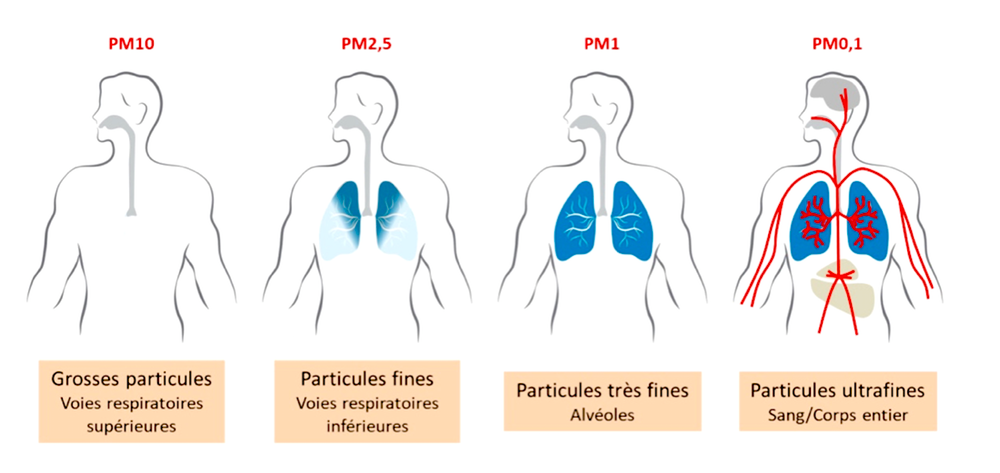
\includegraphics[width=\textwidth]{essence-diesel-fig-2}}
\end{center}

\textbf{Le chauffage au bois en première ligne}\\

Ces particules sont inhalées lors de la respiration et, suivant leur taille, elles peuvent s’accumuler dans les narines, les bronches, les alvéoles pulmonaires ou atteindre les vaisseaux sanguins. On peut considérer que les particules de taille supérieure à 10 microns sont arrêtées par le nez et les voies respiratoires supérieures sans pouvoir pénétrer dans les bronches et les poumons. Mais les particules ultrafines atteignent le réseau sanguin et, avec lui, tous nos organes.
Une étude du CITEPA conduit, pour la France, au classement suivant des sources de PM 2,5~: 9\% pour l’agriculture, 18\% pour le transport routier et 45\% pour le chauffage au bois. Les poids lourds, équipés de moteurs Diesel, sont souvent mis en cause, plus que les voitures et la combustion du bois qui émet pourtant davantage de particules fines. Ce qui est vrai, c’est que les gouttelettes de gazole n’ont pas le temps de s’évaporer avant leur combustion et ne sont que partiellement brûlées ; ceci conduit, entre autres, à la formation de particules, des PM 10 en majorité.
Dans les moteurs à essence, où l’explosion est amorcée par l’étincelle produite par la bougie, la combustion est plus homogène et, en conséquence, les particules produites sont beaucoup plus fines~: PM 2,5, PM 1 et ultrafines. Plus insidieuses puisque plus difficiles à détecter, elles n’en sont pas moins dangereuses.\\

\textbf{Brumes et trajectoires}\\

Il est particulièrement difficile d’extraire ces particules de l’air ambiant où elles servent de germes autour desquels la vapeur d’eau peut se condenser pour former de très fines gouttelettes et donner lieu aux brumes et brouillards.
Lors de la chute d’un objet aussi petit que ces particules ou gouttelettes, le frottement de l’air sur sa surface, dirigé vers le haut, l’emporte sur son poids, dirigé vers le bas. C’est pour cette raison que, comme les particules, les fines gouttelettes de brouillard restent en suspension dans l’air alors que les gouttes de pluie, de taille supérieure à 20 microns, parviennent à tomber.\\

\textbf{48 000 morts par an}\\

Des méthodes statistiques permettent aux épidémiologistes de déceler les corrélations entre la teneur en particules et diverses pathologies ou décès, tout en éliminant l’influence du hasard. Les plus précises conduisent même au mécanisme qui permet à ces particules d’agresser les constituants des cellules de nos organes. Ne citons qu’un seul exemple~: la production d’espèces réactives de l’oxygène qui peuvent l’emporter sur nos mécanismes de défense antioxydants. Au niveau de la paroi des vaisseaux sanguins, un processus inflammatoire, l’athérosclérose, peut alors conduire à un infarctus du myocarde ou à un accident vasculaire cérébral.
Une évaluation quantitative d’impact sanitaire récente conduite par Santé Publique France a établi une relation entre exposition aux PM 2,5 et mortalité.
Cette étude estime que 48 000 décès par an sont imputables à cette pollution par les particules, ce qui correspond à 9\% de la mortalité en France. Elle montre notamment que, si la pollution aux PM 2,5 due aux activités anthropiques était partout la même que dans les communes rurales les moins polluées, 34 000 décès seraient évitables chaque année.
L’augmentation du nombre de décès est liée à l’accroissement de la concentration en PM 25.\\

Pour conclure, rappelons que la plupart des économistes s’accordent pour affirmer que les dépenses qui seraient engendrées par la mise en œuvre de mesures drastiques de réduction de la pollution seraient très inférieures au coût socio-économique engendré par cette même pollution. Ils suivent ainsi Janez Potocnik, Commissaire européen à l’Environnement de 2009 à 2014, qui déclarait~:
«~Si vous pensez que l’économie est plus importante que l’environnement, essayez de retenir votre souffle pendant que vous comptez l’argent.~»


\end{document}


